\section{作业及答案：结构力学基础与技巧班第16次作业及答案（稳定）}
\begin{analysisbox}
稳定问题通常转化为特征值问题。临界荷载由结构刚度退化条件确定，端部约束和有效长度系数是最容易出错的地方。
\end{analysisbox}
\subsection*{第 1 页转写}
四、练习题

11-1图11-24所示刚性杆由两根拉索维持平衡，忽略拉索张力的竖直分量的作用，

则体系的临界荷载为

11-2用静力法求图11-25所示结构的Fper。（北京工业大学2007)

11-3写出图11-26所示压杆稳定的特征方程（EI=常数）。（北京航空航天大学

2008)

El 00

图11-24

图11-25

图11-26

11-4试用静力法求图11-27所示压杆的临界荷载。

11-5求图11-28所示压杆的临界荷载。EI为常数。

11-6求图11-29所示结构的稳定方程（不必求临界荷载）。

461

研究生入学考试辅导丛书结构力学（第二版）

图11-27

图11-28

图11-29

五、练习题答案

Fper

11-1

2a"hEA

(a?+h2)3/2

11-2

Fper

11-3

$\alpha$ltanal=6.

11- 4

[2

11-5

11-6

tanal=
\begin{figure}[H]\centering
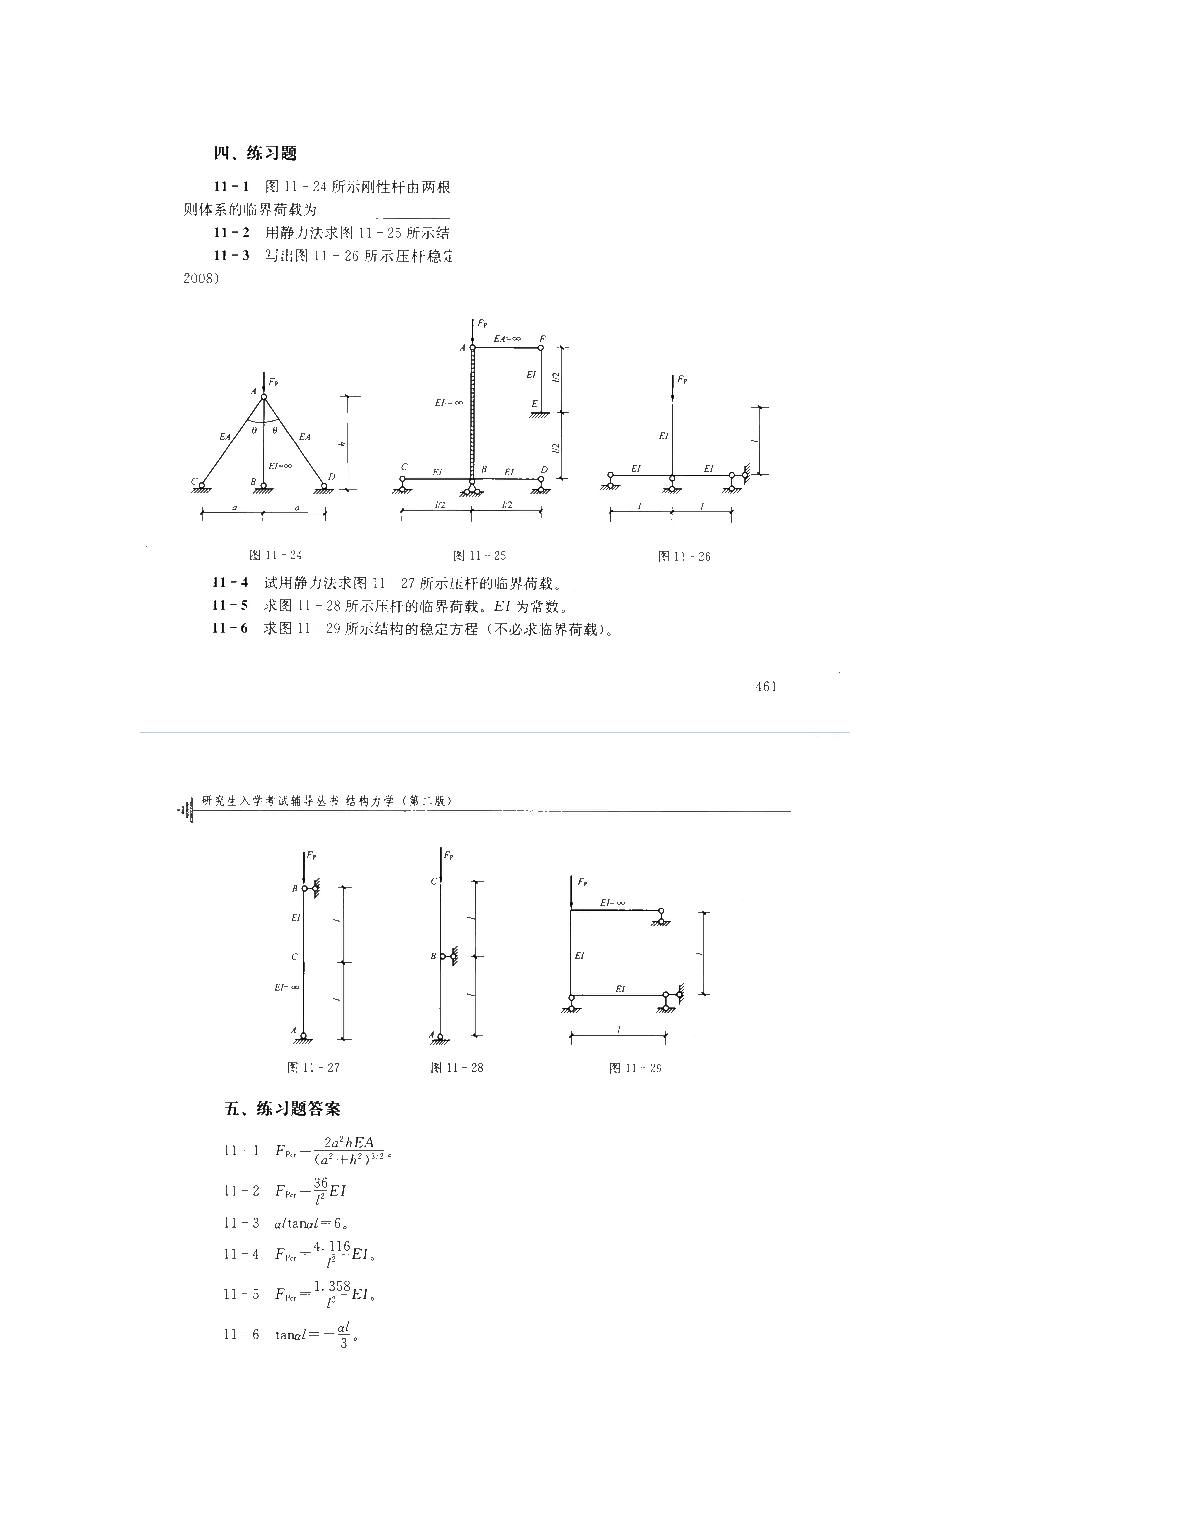
\includegraphics[width=0.92\textwidth]{figures/src19_p001.jpg}
\caption{结构力学基础与技巧班第16次作业及答案（稳定） 第 1 页清理图形页}
\end{figure}
